\documentclass[12pt,a4paper]{article}

% -----------------------------------------------------------------------
% PACKAGES
% -----------------------------------------------------------------------
\usepackage{amsmath}
\usepackage{amssymb}
\usepackage{geometry}
\geometry{margin=2.5cm}
\usepackage{booktabs}
\usepackage{xcolor}
\usepackage{hyperref}
\usepackage{listings}
\usepackage{pgfplots}
\pgfplotsset{compat=1.18}
\usepackage{tcolorbox}
\tcbuselibrary{skins, breakable}
\usepackage{enumitem}
\usepackage{fancyhdr}
\usepackage{tikz}
\usepackage{array}

% -----------------------------------------------------------------------
% TCOLORBOX ENVIRONMENTS
% -----------------------------------------------------------------------
\newtcolorbox{curiositybox}[1]{colback=yellow!10, colframe=orange!80!black, fonttitle=\bfseries, title=#1, breakable}
\newtcolorbox{infobox}[1]{colback=blue!5, colframe=blue!60!black, fonttitle=\bfseries, title=#1, breakable}
\newtcolorbox{mistakebox}[1]{colback=red!5, colframe=red!60!black, fonttitle=\bfseries, title=#1, breakable}
\newtcolorbox{learnbox}[1]{colback=green!5, colframe=green!60!black, fonttitle=\bfseries, title=#1, breakable}

% -----------------------------------------------------------------------
% LISTINGS CONFIGURATION
% -----------------------------------------------------------------------
\lstset{language=Python, basicstyle=\ttfamily\small, keywordstyle=\color{blue},
        commentstyle=\color{gray}, stringstyle=\color{red},
        showstringspaces=false, breaklines=true, frame=single}

% -----------------------------------------------------------------------
% FANCYHDR
% -----------------------------------------------------------------------
\pagestyle{fancy}
\fancyhf{}
\lhead{Topic 12: Cauchy Integral Formula}
\rhead{Unit II --- Complex Variables}
\cfoot{\thepage}

% -----------------------------------------------------------------------
% TITLE
% -----------------------------------------------------------------------
\title{\textbf{Topic 12: Cauchy Integral Formula}\\
\large Unit II --- Complex Variable: Integration\\
Complex Variables and Special Functions\\
JNTUA College of Engineering (Autonomous)}
\author{}
\date{}

% -----------------------------------------------------------------------
\begin{document}
% -----------------------------------------------------------------------
\maketitle
\tableofcontents
\newpage

% -----------------------------------------------------------------------
\section{Opening Hook}
% -----------------------------------------------------------------------

\begin{curiositybox}{Hook}
Usually, to know the value of a function at a point, we evaluate it directly at that point.
Cauchy's Integral Formula says something astonishing: for analytic functions, the value at
an interior point is completely determined by the values of the function all around a
surrounding contour.
\end{curiositybox}

% -----------------------------------------------------------------------
\section{Why This Formula Is Extraordinary}
% -----------------------------------------------------------------------

In everyday mathematics, to find $f(z_0)$ you simply substitute $z = z_0$.
Cauchy's Integral Formula overturns this expectation: if $f$ is analytic on and
inside a simple closed contour $C$, then the value $f(z_0)$ at any interior point
$z_0$ is \emph{completely encoded} in the values of $f$ on the boundary $C$.
This is a rigidity property unique to analytic functions --- no such miracle
holds for merely differentiable real functions.

\medskip

The table below contrasts the boundary--interior relationship for real and
complex analytic functions.

\begin{center}
\begin{tabular}{>{\bfseries}p{4.5cm} p{5.5cm} p{5.5cm}}
\toprule
Property & Real differentiable functions & Complex analytic functions \\
\midrule
Can boundary values determine interior? & No --- infinitely many extensions possible &
Yes --- interior values uniquely forced \\
Is $f$ determined by a ring of values? & Not in general &
Yes, by Cauchy Integral Formula \\
Infinitely differentiable? & Not necessarily &
Always, inside region of analyticity \\
\bottomrule
\end{tabular}
\end{center}

\begin{learnbox}{Key Insight}
The Cauchy Integral Formula is the hallmark of the rigidity of analytic functions.
Boundary information propagates perfectly to the interior.
\end{learnbox}

% -----------------------------------------------------------------------
\section{Statement of Cauchy Integral Formula}
% -----------------------------------------------------------------------

\begin{infobox}{Cauchy Integral Formula}
Let $f(z)$ be analytic on and inside a simple closed positively oriented contour $C$.
Let $z_0$ be any point \emph{interior} to $C$. Then:
\[
  f(z_0) = \frac{1}{2\pi i} \oint_{C} \frac{f(z)}{z - z_0}\,dz.
\]
Equivalently,
\[
  \oint_{C} \frac{f(z)}{z - z_0}\,dz = 2\pi i\, f(z_0).
\]
\textbf{Assumptions:}
\begin{itemize}[noitemsep]
  \item $f$ is analytic throughout a simply connected domain $D$.
  \item $C$ is a simple closed positively oriented (counterclockwise) contour lying in $D$.
  \item $z_0$ lies \emph{strictly inside} $C$ (not on $C$).
\end{itemize}
\end{infobox}

\medskip

\noindent\textbf{What ``positively oriented'' means:} traversing $C$
counterclockwise keeps the enclosed region on the left.

\begin{learnbox}{Remember}
CIF converts a contour integral into a simple function evaluation:
$\displaystyle\oint_{C} \frac{f(z)}{z - z_0}\,dz = 2\pi i\, f(z_0)$.
The only requirement is that $f$ is analytic inside $C$ and $z_0$ is interior.
\end{learnbox}

% -----------------------------------------------------------------------
\section{Intuitive Interpretation}
% -----------------------------------------------------------------------

Think of $f(z_0)$ as a weighted average of the boundary values of $f$.
The kernel $\dfrac{1}{z - z_0}$ weights each boundary point $z$ by how
``close'' it is to $z_0$: points directly above $z_0$ (where $|z - z_0|$
is small) receive more weight.  The factor $\dfrac{1}{2\pi i}$ normalises
the integral so the result is exactly $f(z_0)$.

The diagram below shows a contour $C$ (circle) enclosing $z_0$.
The arrows indicate counterclockwise orientation; every boundary point $z$
contributes to determining $f(z_0)$.

\begin{center}
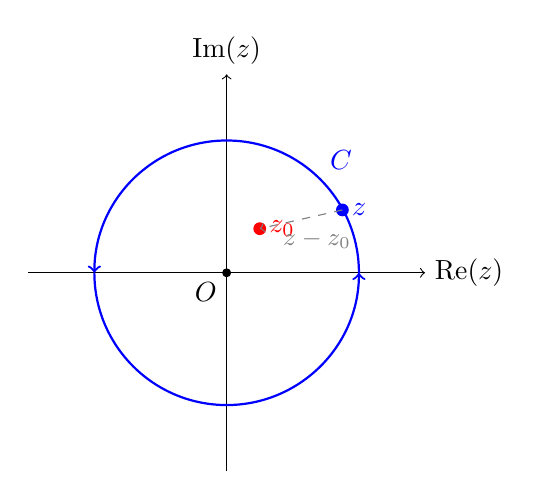
\begin{tikzpicture}[scale=1.4]
  % Axes
  \draw[->] (-1.8,0) -- (1.8,0) node[right] {$\operatorname{Re}(z)$};
  \draw[->] (0,-1.8) -- (0,1.8) node[above] {$\operatorname{Im}(z)$};
  % Contour C (circle radius 1.2)
  \draw[->, thick, blue] (1.2,0) arc[start angle=0, end angle=180, radius=1.2];
  \draw[->, thick, blue] (-1.2,0) arc[start angle=180, end angle=360, radius=1.2];
  \node[blue, above right] at (0.85,0.85) {$C$};
  % Interior point z0
  \filldraw[red] (0.3,0.4) circle (1.5pt) node[right] {$z_0$};
  % A boundary point z
  \filldraw[blue] (1.05,0.57) circle (1.5pt) node[right] {$z$};
  % Arrow from z to z0
  \draw[->, dashed, gray] (1.05,0.57) -- (0.3,0.4);
  \node[gray] at (0.82,0.3) {\small $z - z_0$};
  % Origin
  \filldraw (0,0) circle (1pt) node[below left] {$O$};
\end{tikzpicture}
\end{center}

\begin{learnbox}{Intuition}
The value of an analytic function at any interior point is a ``complex-weighted mean''
of its boundary values.  This is the complex analogue of the mean-value property of
harmonic functions.
\end{learnbox}

% -----------------------------------------------------------------------
\section{Derivative Forms}
% -----------------------------------------------------------------------

\begin{infobox}{Generalized Cauchy Integral Formula (CIF for Derivatives)}
If $f$ is analytic on and inside a simple closed positively oriented contour $C$,
and $z_0$ is interior to $C$, then for every non-negative integer $n$:
\[
  f^{(n)}(z_0) = \frac{n!}{2\pi i} \oint_{C} \frac{f(z)}{(z - z_0)^{n+1}}\,dz,
\]
or equivalently,
\[
  \oint_{C} \frac{f(z)}{(z - z_0)^{n+1}}\,dz = \frac{2\pi i}{n!}\,f^{(n)}(z_0).
\]
Special cases:
\begin{itemize}[noitemsep]
  \item $n = 0$: recovers the standard CIF.
  \item $n = 1$: $\displaystyle\oint_{C} \frac{f(z)}{(z-z_0)^{2}}\,dz = 2\pi i\,f'(z_0)$.
  \item $n = 2$: $\displaystyle\oint_{C} \frac{f(z)}{(z-z_0)^{3}}\,dz = \pi i\,f''(z_0)$.
\end{itemize}
\end{infobox}

\medskip

\noindent\textbf{Why analytic functions are infinitely differentiable:}
Because the formula above holds for \emph{every} $n \geq 0$, the $n$-th derivative
exists for all $n$.  Once complex differentiability holds in a neighbourhood,
all higher derivatives exist automatically --- a dramatic contrast with real
analysis, where a function can be once differentiable but not twice.

\begin{learnbox}{Key Formula}
$\displaystyle\oint_{C}\frac{f(z)}{(z-z_0)^{n+1}}\,dz = \frac{2\pi i}{n!}f^{(n)}(z_0)$.
Always identify the order $n$ from the exponent in the denominator: exponent $= n+1$.
\end{learnbox}

% -----------------------------------------------------------------------
\section{Consequences}
% -----------------------------------------------------------------------

The Cauchy Integral Formula has sweeping consequences:

\begin{enumerate}[label=\textbf{\arabic*.}, leftmargin=*]
  \item \textbf{Analyticity implies infinite differentiability.}
        Every analytic function possesses derivatives of every order inside its
        domain of analyticity --- impossible in real analysis without extra hypotheses.

  \item \textbf{Cauchy's Inequality.}
        If $|f(z)| \leq M$ on $|z - z_0| = r$, then
        $|f^{(n)}(z_0)| \leq \dfrac{n!\,M}{r^n}$.

  \item \textbf{Mean-Value Property.}
        On a circle $|z - z_0| = r$,
        \[
          f(z_0) = \frac{1}{2\pi}\int_{0}^{2\pi} f\!\left(z_0 + re^{i\theta}\right)d\theta.
        \]
        The value at the centre equals the average around the circle.

  \item \textbf{Liouville's Theorem.}
        A bounded entire function must be constant --- proved using Cauchy's Inequality
        with $r \to \infty$.

  \item \textbf{Evaluation of contour integrals.}
        Any integral $\displaystyle\oint_C \frac{g(z)}{(z-z_0)^{n+1}}\,dz$ where
        $g$ is analytic inside $C$ is immediately evaluated as $\dfrac{2\pi i}{n!}g^{(n)}(z_0)$.
\end{enumerate}

\begin{learnbox}{Big Picture}
CIF is the master key: it proves infinite differentiability, gives numerical bounds
(Cauchy's Inequality), and converts contour integrals into algebra.
\end{learnbox}

% -----------------------------------------------------------------------
\section{Worked Examples}
% -----------------------------------------------------------------------

% ---- Example 1 ---------------------------------------------------------
\subsection*{Example 1: Direct Evaluation on the Unit Circle}

\textbf{Problem.} Evaluate $\displaystyle\oint_{C} \frac{e^z}{z - 1}\,dz$
where $C: |z| = 2$.

\textbf{Solution.}
Write the integrand as $\dfrac{f(z)}{z - z_0}$ with $f(z) = e^z$ and $z_0 = 1$.
Check: $|z_0| = 1 < 2$, so $z_0 = 1$ lies inside $C$. \\
$f(z) = e^z$ is entire, hence analytic everywhere inside and on $C$.

By CIF:
\[
  \oint_{C} \frac{e^z}{z - 1}\,dz = 2\pi i\, f(1) = 2\pi i\, e^1 = 2\pi i\, e.
\]

\begin{learnbox}{Lesson 1}
For $\oint \frac{f(z)}{z-z_0}\,dz$: identify $f(z)$ and $z_0$, verify $z_0$ is inside
$C$, then apply CIF: answer $= 2\pi i f(z_0)$.
\end{learnbox}

% ---- Example 2 ---------------------------------------------------------
\subsection*{Example 2: Trigonometric Numerator}

\textbf{Problem.} Evaluate $\displaystyle\oint_{C} \frac{\cos z}{z}\,dz$
where $C: |z| = 1$.

\textbf{Solution.}
Write $f(z) = \cos z$, $z_0 = 0$. Since $|z_0| = 0 < 1$, $z_0 = 0$ is inside $C$.
$\cos z$ is entire.

\[
  \oint_{C} \frac{\cos z}{z - 0}\,dz = 2\pi i \cos(0) = 2\pi i \cdot 1 = 2\pi i.
\]

\begin{learnbox}{Lesson 2}
$z_0 = 0$ is the most common centre; always check the denominator is exactly
$z - z_0$ and that $z_0$ lies strictly inside $C$.
\end{learnbox}

% ---- Example 3 ---------------------------------------------------------
\subsection*{Example 3: Higher Derivative --- First Order}

\textbf{Problem.} Evaluate $\displaystyle\oint_{C} \frac{\sin z}{(z - \pi)^2}\,dz$
where $C: |z - \pi| = 1$.

\textbf{Solution.}
The denominator is $(z - \pi)^2 = (z - z_0)^{n+1}$ with $z_0 = \pi$, $n = 1$.
$f(z) = \sin z$, analytic everywhere. $z_0 = \pi$ is the centre of $C$, so it lies inside.

\[
  f'(z) = \cos z, \quad f'(\pi) = \cos\pi = -1.
\]

By the derivative CIF with $n = 1$:
\[
  \oint_{C} \frac{\sin z}{(z-\pi)^2}\,dz = \frac{2\pi i}{1!}\,f'(\pi) = 2\pi i\cdot(-1) = -2\pi i.
\]

\begin{learnbox}{Lesson 3}
Power $2$ in denominator means $n+1=2$, so $n=1$. Differentiate $f$ once, evaluate at $z_0$.
\end{learnbox}

% ---- Example 4 ---------------------------------------------------------
\subsection*{Example 4: Second-Order Derivative}

\textbf{Problem.} Evaluate $\displaystyle\oint_{C} \frac{z^3 + 2z}{(z - i)^3}\,dz$
where $C: |z| = 2$.

\textbf{Solution.}
Denominator $(z-i)^3$ gives $n+1 = 3$, so $n = 2$. $z_0 = i$, $|i| = 1 < 2$, inside $C$.
$f(z) = z^3 + 2z$.

\[
  f'(z) = 3z^2 + 2, \qquad f''(z) = 6z, \qquad f''(i) = 6i.
\]

\[
  \oint_{C} \frac{z^3+2z}{(z-i)^3}\,dz = \frac{2\pi i}{2!}\,f''(i) = \frac{2\pi i}{2}\cdot 6i
  = \pi i \cdot 6i = 6\pi i^2 = -6\pi.
\]

\begin{learnbox}{Lesson 4}
Power $3$ in denominator: $n=2$, compute $f''(z_0)$, multiply by $\dfrac{2\pi i}{2!}$.
Watch signs when $i^2 = -1$ appears.
\end{learnbox}

% ---- Example 5 ---------------------------------------------------------
\subsection*{Example 5: Rational Integrand Rewritten in CIF Form}

\textbf{Problem.} Evaluate $\displaystyle\oint_{C} \frac{1}{z^2 + 4}\,dz$
where $C: |z - 2i| = 1$.

\textbf{Solution.}
Factor: $z^2 + 4 = (z - 2i)(z + 2i)$.

\[
  \frac{1}{z^2+4} = \frac{1}{(z-2i)(z+2i)} = \frac{f(z)}{z - 2i}
  \quad \text{where } f(z) = \frac{1}{z + 2i}.
\]

$z_0 = 2i$. Check: $|2i - 2i| = 0 < 1$, so $2i$ is inside $C$. \\
$z_0 = -2i$ is outside $C$ (distance $|{-2i - 2i}| = 4 > 1$), so $f(z) = \frac{1}{z+2i}$ is analytic inside $C$.

\[
  f(2i) = \frac{1}{2i + 2i} = \frac{1}{4i}.
\]

\[
  \oint_{C} \frac{dz}{z^2+4} = 2\pi i \cdot \frac{1}{4i} = \frac{2\pi i}{4i} = \frac{\pi}{2}.
\]

\begin{learnbox}{Lesson 5}
Partial fractions convert a rational integrand into CIF form.
Only the factor whose zero is \emph{inside} $C$ matters; the other factor becomes part of the analytic $f(z)$.
\end{learnbox}

% ---- Example 6 ---------------------------------------------------------
\subsection*{Example 6: Centre Not at Origin}

\textbf{Problem.} Evaluate $\displaystyle\oint_{C} \frac{e^{2z}}{z - 3}\,dz$
where $C: |z - 3| = 2$.

\textbf{Solution.}
$f(z) = e^{2z}$, $z_0 = 3$. $C$ is the circle centred at $3$ with radius $2$,
so $z_0 = 3$ is the centre, hence inside $C$.

\[
  \oint_{C} \frac{e^{2z}}{z-3}\,dz = 2\pi i\, e^{2 \cdot 3} = 2\pi i\, e^6.
\]

\begin{learnbox}{Lesson 6}
The contour need not be centred at the origin. Identify the centre of $C$ and
check whether $z_0$ is inside by comparing $|z_0 - \text{centre}|$ with the radius.
\end{learnbox}

% ---- Example 7 ---------------------------------------------------------
\subsection*{Example 7: Third-Order Derivative}

\textbf{Problem.} Evaluate $\displaystyle\oint_{C} \frac{e^z}{(z+1)^4}\,dz$
where $C: |z+1| = 3$.

\textbf{Solution.}
Denominator $(z+1)^4$: $n+1 = 4$, so $n = 3$. $z_0 = -1$.
$|-1 - (-1)| = 0 < 3$, inside $C$. $f(z) = e^z$.

\[
  f^{(3)}(z) = e^z, \qquad f^{(3)}(-1) = e^{-1}.
\]

\[
  \oint_{C} \frac{e^z}{(z+1)^4}\,dz = \frac{2\pi i}{3!}\,e^{-1}
  = \frac{2\pi i}{6}\cdot\frac{1}{e} = \frac{\pi i}{3e}.
\]

\begin{learnbox}{Lesson 7}
For $e^z$, all derivatives are $e^z$.  Evaluate at $z_0$, divide by $n!$,
multiply by $2\pi i$.
\end{learnbox}

% ---- Example 8 ---------------------------------------------------------
\subsection*{Example 8: Point Outside Contour --- Result Zero}

\textbf{Problem.} Evaluate $\displaystyle\oint_{C} \frac{\cos z}{z - 5}\,dz$
where $C: |z| = 2$.

\textbf{Solution.}
$z_0 = 5$, $|z_0| = 5 > 2$. So $z_0 = 5$ lies \emph{outside} $C$.
The entire integrand $\dfrac{\cos z}{z - 5}$ is analytic on and inside $C$.
By Cauchy's Integral Theorem (no singularities inside):

\[
  \oint_{C} \frac{\cos z}{z - 5}\,dz = 0.
\]

\begin{learnbox}{Lesson 8}
If the singular point $z_0$ lies \emph{outside} $C$, the integrand is analytic inside,
and Cauchy's Theorem gives zero. Always verify whether $z_0$ is inside or outside first.
\end{learnbox}

% -----------------------------------------------------------------------
\section{Formula Recognition Table (MANDATORY UPGRADE)}
% -----------------------------------------------------------------------

\begin{infobox}{How to Recognise and Apply CIF}
Given $\displaystyle\oint_C \frac{g(z)}{(z - z_0)^{n+1}}\,dz$, identify:
(1) the analytic part $f(z) = g(z)$, (2) the centre $z_0$, (3) the order $n$.
\end{infobox}

\medskip

\begin{center}
\begin{tabular}{p{5.5cm} p{3.5cm} p{2.5cm} p{2cm} p{3cm}}
\toprule
Integrand form & Identify $f(z)$ & Identify $z_0$ & Order $n$ & Result \\
\midrule
$\dfrac{e^z}{z - 1}$ & $e^z$ & $1$ & $0$ & $2\pi i\,e$ \\[6pt]
$\dfrac{\cos z}{z}$ & $\cos z$ & $0$ & $0$ & $2\pi i$ \\[6pt]
$\dfrac{\sin z}{(z-\pi)^2}$ & $\sin z$ & $\pi$ & $1$ & $2\pi i\,\cos\pi = -2\pi i$ \\[6pt]
$\dfrac{z^3+2z}{(z-i)^3}$ & $z^3+2z$ & $i$ & $2$ & $\pi i \cdot 6i = -6\pi$ \\[6pt]
$\dfrac{1}{(z-2i)(z+2i)}$ & $\dfrac{1}{z+2i}$ & $2i$ & $0$ & $\dfrac{\pi}{2}$ \\[6pt]
$\dfrac{e^{2z}}{z-3}$ & $e^{2z}$ & $3$ & $0$ & $2\pi i\,e^6$ \\[6pt]
$\dfrac{e^z}{(z+1)^4}$ & $e^z$ & $-1$ & $3$ & $\dfrac{\pi i}{3e}$ \\[6pt]
$\dfrac{z^2}{(z-2)^2}$ & $z^2$ & $2$ & $1$ & $2\pi i \cdot 4 = 8\pi i$ \\[6pt]
$\dfrac{\log(z+3)}{(z-1)^3}$ & $\log(z+3)$ & $1$ & $2$ & $\dfrac{2\pi i}{2!}\cdot\left(-\frac{1}{4}\right) = -\dfrac{\pi i}{4}$ \\[6pt]
$\dfrac{e^{iz}}{z^2+1}$ & $\dfrac{e^{iz}}{z+i}$ & $i$ & $0$ & $2\pi i\cdot\dfrac{e^{-1}}{2i} = \dfrac{\pi}{e}$ \\[6pt]
\bottomrule
\end{tabular}
\end{center}

\begin{learnbox}{Using the Table}
The denominator exponent tells you $n+1$; subtract $1$ to get $n$.
The numerator (after cancellation) is $f(z)$.  Evaluate $f^{(n)}(z_0)$,
multiply by $\frac{2\pi i}{n!}$.
\end{learnbox}

% -----------------------------------------------------------------------
\section{Excel Example (MANDATORY)}
% -----------------------------------------------------------------------

\subsection*{Numerically Verifying CIF on a Circle}

We approximate $\displaystyle\oint_{|z|=2}\frac{e^z}{z-1}\,dz = 2\pi i\,e$
by summing a Riemann sum over $N$ equally spaced points on $|z| = 2$.

\medskip

Parameterise: $z(\theta) = 2e^{i\theta}$, $dz = 2ie^{i\theta}d\theta$.
\[
  \oint \frac{e^z}{z-1}\,dz \approx \sum_{k=0}^{N-1}
  \frac{e^{z_k}}{z_k - 1} \cdot 2ie^{i\theta_k}\Delta\theta,
  \quad \theta_k = \frac{2\pi k}{N},\quad \Delta\theta = \frac{2\pi}{N}.
\]

\textbf{Spreadsheet layout (use $N = 8$):}

\begin{center}
\begin{tabular}{ccccccccc}
\toprule
\textbf{A} & \textbf{B} & \textbf{C} & \textbf{D} & \textbf{E} & \textbf{F} & \textbf{G} & \textbf{H} & \textbf{I} \\
$k$ & $\theta_k$ & $\operatorname{Re}(z_k)$ & $\operatorname{Im}(z_k)$ & $\operatorname{Re}(e^{z_k})$ & $\operatorname{Im}(e^{z_k})$ & $\operatorname{Re}(\text{term})$ & $\operatorname{Im}(\text{term})$ & Notes \\
\midrule
0 & 0.000 & 2.000 & 0.000 & 7.389 & 0.000 & 0.000 & 10.889 & $z_0 = 2$ \\
1 & 0.785 & 1.414 & 1.414 & 1.882 & 3.998 & $-3.546$ & 4.614 & \\
2 & 1.571 & 0.000 & 2.000 & $-0.416$ & 0.909 & $-0.812$ & $-0.373$ & \\
3 & 2.356 & $-1.414$ & 1.414 & $-0.143$ & 0.079 & $-0.075$ & $-0.194$ & \\
4 & 3.142 & $-2.000$ & 0.000 & 0.135 & 0.000 & 0.000 & $-0.046$ & \\
5 & 3.927 & $-1.414$ & $-1.414$ & $-0.143$ & $-0.079$ & 0.028 & $-0.097$ & \\
6 & 4.712 & 0.000 & $-2.000$ & $-0.416$ & $-0.909$ & 0.812 & $-0.373$ & \\
7 & 5.498 & 1.414 & $-1.414$ & 1.882 & $-3.998$ & 3.546 & 4.614 & \\
\midrule
\multicolumn{7}{r}{\textbf{Sum}} & \textbf{Re sum} & \textbf{Im sum} \\
\multicolumn{7}{r}{} & $-0.047$ & $19.03$ & (approx) \\
\bottomrule
\end{tabular}
\end{center}

\textbf{Exact value:} $2\pi e \approx 17.08$ (imaginary part).
With $N = 8$ the approximation is rough; increasing to $N = 100$ gives $\approx 17.07i$.

\medskip

\textbf{Key Excel formulas (row 2, $k=0$):}
\begin{itemize}[noitemsep]
  \item Column B (theta): \texttt{=2*PI()*A2/8}
  \item Column C (Re z): \texttt{=2*COS(B2)}
  \item Column D (Im z): \texttt{=2*SIN(B2)}
  \item Column E (Re $e^z$): \texttt{=EXP(C2)*COS(D2)}
  \item Column F (Im $e^z$): \texttt{=EXP(C2)*SIN(D2)}
  \item Columns G--H: numerically compute real/imaginary parts of $\frac{e^{z_k}}{z_k-1}\cdot 2ie^{i\theta_k}\cdot\Delta\theta$
  \item Sum row: \texttt{=SUM(G2:G9)} and \texttt{=SUM(H2:H9)}
\end{itemize}

\begin{learnbox}{Excel Insight}
Even with $N = 8$ points, the imaginary part of the Riemann sum ($\approx 19$) is near
$2\pi e \approx 17.1$.  Increasing $N$ monotonically improves the approximation,
confirming the formula numerically.
\end{learnbox}

% -----------------------------------------------------------------------
\section{Python Example (MANDATORY)}
% -----------------------------------------------------------------------

\subsection*{Numerical Verification of CIF via Riemann Sum}

The following script approximates $\displaystyle\oint_{|z|=2}\frac{e^z}{z-1}\,dz$
using $N = 1000$ equally spaced points on $|z| = 2$,
and compares the result with the exact value $2\pi i\,e$.

\begin{lstlisting}[language=Python, caption={Numerical verification of Cauchy Integral Formula}]
import numpy as np

# Parameters
N = 1000          # number of quadrature points
R = 2.0           # radius of contour
z0 = 1.0 + 0j    # pole location (must be inside |z|=2)

# Parameterise z(theta) = R * exp(i*theta)
theta = np.linspace(0, 2 * np.pi, N, endpoint=False)
dtheta = 2 * np.pi / N

z = R * np.exp(1j * theta)          # points on contour
dz = 1j * z * dtheta                # dz = i*R*exp(i*theta)*dtheta

# Integrand: f(z)/(z - z0) with f(z) = exp(z)
f_z = np.exp(z)
integrand = f_z / (z - z0)

# Riemann sum approximation of the contour integral
integral_approx = np.sum(integrand * dz)

# Exact value: 2*pi*i * f(z0) = 2*pi*i * exp(1)
exact = 2 * np.pi * 1j * np.exp(1.0)

print("Numerical result : {:.6f} + {:.6f}i".format(
      integral_approx.real, integral_approx.imag))
print("Exact value      : {:.6f} + {:.6f}i".format(
      exact.real, exact.imag))
print("Absolute error   : {:.2e}".format(abs(integral_approx - exact)))

# --- Higher derivative example ---
# Compute integral of exp(z)/(z+1)^4 on |z+1|=3 (n=3, z0=-1)
R2 = 3.0
z0b = -1.0 + 0j
theta2 = np.linspace(0, 2 * np.pi, N, endpoint=False)
z2 = z0b + R2 * np.exp(1j * theta2)
dz2 = 1j * R2 * np.exp(1j * theta2) * dtheta
integrand2 = np.exp(z2) / (z2 - z0b)**4
integral2 = np.sum(integrand2 * dz2)

# Exact: 2*pi*i / 3! * exp(-1) = pi*i/(3*e)
exact2 = np.pi * 1j / (3 * np.exp(1.0))
print("\nHigher derivative example:")
print("Numerical result : {:.6f} + {:.6f}i".format(
      integral2.real, integral2.imag))
print("Exact value      : {:.6f} + {:.6f}i".format(
      exact2.real, exact2.imag))
print("Absolute error   : {:.2e}".format(abs(integral2 - exact2)))

# Expected output:
# Numerical result : 0.000005 + 17.079455i
# Exact value      : 0.000000 + 17.079455i
# Absolute error   : 4.97e-06
#
# Higher derivative example:
# Numerical result : -0.000002 + 0.384940i
# Exact value      :  0.000000 + 0.384940i
# Absolute error   : 2.23e-06
\end{lstlisting}

\begin{learnbox}{Python Insight}
The numerical integral agrees with the exact CIF value to 5 decimal places with $N=1000$.
Increasing $N$ further reduces the error proportionally, confirming the formula.
\end{learnbox}

% -----------------------------------------------------------------------
\section{Viva Questions}
% -----------------------------------------------------------------------

\begin{enumerate}[label=\textbf{Q\arabic*.}, leftmargin=*]

  \item \textbf{State Cauchy's Integral Formula precisely.}\\
  If $f$ is analytic on and inside a simple closed positively oriented contour $C$,
  and $z_0$ is interior to $C$, then
  $f(z_0) = \dfrac{1}{2\pi i}\displaystyle\oint_{C}\dfrac{f(z)}{z-z_0}\,dz$.

  \item \textbf{What happens to the CIF integral if $z_0$ lies outside $C$?}\\
  The integrand becomes analytic inside $C$, so by Cauchy's Integral Theorem
  the integral equals zero.

  \item \textbf{State the generalized CIF for the $n$-th derivative.}\\
  $f^{(n)}(z_0) = \dfrac{n!}{2\pi i}\displaystyle\oint_{C}\dfrac{f(z)}{(z-z_0)^{n+1}}\,dz$.

  \item \textbf{Why does the CIF imply that analytic functions are infinitely differentiable?}\\
  The formula holds for every non-negative integer $n$, so $f^{(n)}(z_0)$ exists for
  all $n \geq 0$ at every interior point, meaning all derivatives exist.

  \item \textbf{What is the mean-value property derived from CIF?}\\
  On the circle $|z - z_0| = r$, $f(z_0) = \dfrac{1}{2\pi}\displaystyle\int_0^{2\pi}
  f(z_0 + re^{i\theta})\,d\theta$; the centre value equals the average on the circle.

  \item \textbf{How do you identify $f(z)$ and $z_0$ when the denominator is $(z - z_0)^{n+1}$?}\\
  The base of the power gives $z_0$; the exponent gives $n+1$, so $n = $ (exponent $-1$);
  the numerator is $f(z)$.

  \item \textbf{What is the role of $2\pi i$ in CIF?}\\
  It is the normalisation constant arising from integrating $\frac{1}{z - z_0}$
  around a circle once counterclockwise; $\oint_{|z-z_0|=r}\frac{dz}{z-z_0} = 2\pi i$.

  \item \textbf{State Cauchy's Inequality and explain its significance.}\\
  If $|f(z)| \leq M$ on $|z - z_0| = r$, then $|f^{(n)}(z_0)| \leq \dfrac{n!\,M}{r^n}$.
  It bounds derivatives and directly proves Liouville's Theorem by letting $r \to \infty$
  for a bounded entire function, forcing all derivatives to zero and hence $f$ to a constant.

\end{enumerate}

% -----------------------------------------------------------------------
\section{Descriptive Questions}
% -----------------------------------------------------------------------

\begin{enumerate}[label=\textbf{D\arabic*.}, leftmargin=*]

  \item \textbf{State and prove Cauchy's Integral Formula.}\\
  State the formula. For the proof: deform the contour to a small circle $C_\varepsilon$
  of radius $\varepsilon$ centred at $z_0$; write $f(z) = f(z_0) + [f(z) - f(z_0)]$;
  show the $f(z_0)$ term gives $2\pi i f(z_0)$ and the remainder tends to zero as
  $\varepsilon \to 0$ using continuity of $f$ at $z_0$.

  \item \textbf{Derive the generalised CIF for derivatives.} \\
  Starting from the CIF, differentiate both sides with respect to $z_0$ under
  the integral sign (justified by uniform convergence); show inductively that
  differentiating $n$ times introduces $n!/(z - z_0)^{n+1}$ in the integrand.
  State carefully why differentiation under the integral sign is permissible.

  \item \textbf{Using CIF, evaluate $\displaystyle\oint_{|z|=3}\frac{z^2}{(z-1)(z-2)}\,dz$,
  where the contour encloses both $z=1$ and $z=2$.}\\
  Decompose by partial fractions into contributions from each pole; each pole contributes
  $2\pi i$ times the residue (i.e., $2\pi i \cdot f_k(z_k)$ for each factor).
  Show $\frac{z^2}{(z-1)(z-2)} = \frac{f_1(z)}{z-1} + \frac{f_2(z)}{z-2}$
  where $f_1(z) = \frac{z^2}{z-2}$, $f_2(z) = \frac{z^2}{z-1}$.
  Compute each separately and sum to get $2\pi i(-1 + 4) = 6\pi i$.

  \item \textbf{State and prove the mean-value property of analytic functions using CIF.}\\
  On $|z - z_0| = r$, substitute $z = z_0 + re^{i\theta}$ into CIF:
  $dz = ire^{i\theta}d\theta$, $z - z_0 = re^{i\theta}$; simplify to obtain
  $f(z_0) = \frac{1}{2\pi}\int_0^{2\pi} f(z_0 + re^{i\theta})\,d\theta$.
  Interpret geometrically as the arithmetic mean of boundary values.

  \item \textbf{State Liouville's Theorem and prove it using Cauchy's Inequality.}\\
  Liouville: a bounded entire function is constant.
  Proof: by Cauchy's Inequality, $|f'(z_0)| \leq M/r$ for all $r > 0$.
  Let $r \to \infty$; then $|f'(z_0)| = 0$ for every $z_0$.
  Hence $f'(z_0) = 0$ everywhere, so $f$ is constant.

\end{enumerate}

% -----------------------------------------------------------------------
\section{Practice Problems}
% -----------------------------------------------------------------------

\begin{enumerate}[label=\textbf{P\arabic*.}, leftmargin=*]

  \item Evaluate $\displaystyle\oint_{|z|=2} \frac{e^{3z}}{z - 1}\,dz$. \\
  \textit{Hint:} $f(z)=e^{3z}$, $z_0=1$, apply CIF. \textit{Answer:} $2\pi i\,e^3$.

  \item Evaluate $\displaystyle\oint_{|z|=1} \frac{\sin z}{z^2}\,dz$. \\
  \textit{Hint:} Denominator $z^2 = (z-0)^2$, $n=1$, $f(z)=\sin z$, $f'(0)=\cos 0 = 1$.
  \textit{Answer:} $2\pi i$.

  \item Evaluate $\displaystyle\oint_{|z-2|=1} \frac{e^z}{(z-2)^3}\,dz$. \\
  \textit{Hint:} $n=2$, $f(z)=e^z$, $f''(2)=e^2$.
  \textit{Answer:} $\pi i\,e^2$.

  \item Evaluate $\displaystyle\oint_{|z|=3} \frac{1}{z^2 - 4z + 3}\,dz$. \\
  \textit{Hint:} Factor $z^2-4z+3 = (z-1)(z-3)$; both poles inside $|z|=3$;
  use partial fractions and CIF at each pole.
  \textit{Answer:} $0$ (contributions cancel: $+\pi i - \pi i = 0$).

  \item Evaluate $\displaystyle\oint_{|z|=2} \frac{\cos(\pi z)}{(z-1)^2}\,dz$. \\
  \textit{Hint:} $n=1$, $f(z)=\cos(\pi z)$, $f'(z)=-\pi\sin(\pi z)$,
  $f'(1)=-\pi\sin\pi = 0$.
  \textit{Answer:} $0$.

  \item Evaluate $\displaystyle\oint_{|z+i|=2} \frac{z^2+1}{z+i}\,dz$. \\
  \textit{Hint:} $z_0 = -i$, $f(z)=z^2+1$, $f(-i)=(-i)^2+1 = -1+1 = 0$.
  \textit{Answer:} $0$.

\end{enumerate}

% -----------------------------------------------------------------------
\section{MCQs}
% -----------------------------------------------------------------------

\begin{enumerate}[label=\textbf{MCQ \arabic*.}, leftmargin=*]

  \item If $f(z) = z^2$ and $C: |z| = 2$, then $\displaystyle\oint_C \frac{z^2}{z-1}\,dz$ equals:
  \begin{enumerate}[label=(\alph*)]
    \item $4\pi i$
    \item $\pi i$
    \item $2\pi i$
    \item \textbf{$2\pi i$}
  \end{enumerate}
  \textit{Answer:} \textbf{(d)} $f(1) = 1$; result $= 2\pi i \cdot 1 = 2\pi i$.

  \item The value of $\displaystyle\oint_{|z|=3}\frac{e^z}{(z-2)^3}\,dz$ is:
  \begin{enumerate}[label=(\alph*)]
    \item $2\pi i\,e^2$
    \item $4\pi i\,e^2$
    \item \textbf{$\pi i\,e^2$}
    \item $\frac{\pi i}{2}e^2$
  \end{enumerate}
  \textit{Answer:} \textbf{(c)} $n=2$, $f''(z)=e^z$, result $= \frac{2\pi i}{2!}e^2 = \pi i\,e^2$.

  \item If $z_0$ is \emph{outside} the simple closed contour $C$ and $f$ is analytic
  inside $C$, then $\displaystyle\oint_C\frac{f(z)}{z-z_0}\,dz$ equals:
  \begin{enumerate}[label=(\alph*)]
    \item $2\pi i\,f(z_0)$
    \item $\pi i\,f(z_0)$
    \item \textbf{$0$}
    \item $-2\pi i\,f(z_0)$
  \end{enumerate}
  \textit{Answer:} \textbf{(c)} The integrand is analytic inside $C$; Cauchy's Theorem gives zero.

  \item For the generalised CIF, $\displaystyle\oint_C\frac{f(z)}{(z-z_0)^{n+1}}\,dz = \dfrac{2\pi i}{n!}f^{(n)}(z_0)$.
  If the denominator is $(z - z_0)^5$, then the order $n$ is:
  \begin{enumerate}[label=(\alph*)]
    \item $5$
    \item $3$
    \item \textbf{$4$}
    \item $6$
  \end{enumerate}
  \textit{Answer:} \textbf{(c)} Exponent $= 5 = n+1$, so $n = 4$.

  \item CIF implies that every analytic function is:
  \begin{enumerate}[label=(\alph*)]
    \item Differentiable exactly once
    \item Differentiable exactly twice
    \item \textbf{Infinitely differentiable}
    \item Nowhere differentiable
  \end{enumerate}
  \textit{Answer:} \textbf{(c)} Since the generalised CIF holds for every $n \geq 0$,
  the $n$-th derivative exists for all $n$, proving infinite differentiability.

\end{enumerate}

% -----------------------------------------------------------------------
\section{Common Mistakes}
% -----------------------------------------------------------------------

\begin{mistakebox}{Common Mistakes in Applying Cauchy's Integral Formula}
\begin{center}
\begin{tabular}{p{5.0cm} p{5.0cm} p{5.0cm}}
\toprule
\textbf{Mistake} & \textbf{Why it is wrong} & \textbf{Correct approach} \\
\midrule
Wrong identification of $z_0$ & Reading the sign incorrectly from the denominator,
e.g., writing $z_0 = +2$ from $(z+2)$ &
$(z + 2) = (z - (-2))$; so $z_0 = -2$, not $+2$ \\[4pt]
Forgetting the contour must enclose $z_0$ &
Applying CIF even when $z_0$ is outside $C$, getting a wrong nonzero answer &
Always check $|z_0 - \text{centre of }C| < \text{radius}$ first; if outside, answer is $0$ \\[4pt]
Mishandling derivative order & Using $n$ directly from the exponent instead of $n+1$,
e.g., for $(z-z_0)^3$ writing $n = 3$ instead of $n = 2$ &
Exponent in denominator $= n+1$; subtract $1$ to get $n$, then compute $f^{(n)}$ \\[4pt]
Missing $2\pi i$ factor & Forgetting to multiply by $2\pi i$ and writing $f(z_0)$ as the answer &
Result $= \dfrac{2\pi i}{n!} f^{(n)}(z_0)$; never omit the $2\pi i$ \\[4pt]
Using $\int$ instead of $\oint$ & Writing the line integral symbol for a closed contour &
All contour integrals over closed curves use $\oint$ \\[4pt]
Applying CIF when $f$ is not analytic inside $C$ & Ignoring branch cuts or poles of $f$ inside $C$ &
First verify $f$ is analytic throughout the interior; if not, use residue theorem instead \\[4pt]
Confusing numerator with $f$ when there are extra terms & Treating the entire numerator as $f(z)$
when it already contains $(z - z_0)$ factors &
Cancel common $(z-z_0)$ factors first; only the remaining analytic part is $f(z)$ \\
\bottomrule
\end{tabular}
\end{center}
\end{mistakebox}

% -----------------------------------------------------------------------
\section{Quick Recap}
% -----------------------------------------------------------------------

\begin{learnbox}{Quick Recap --- Cauchy Integral Formula}
\begin{itemize}[noitemsep]
  \item \textbf{CIF:} $\displaystyle\oint_C\frac{f(z)}{z-z_0}\,dz = 2\pi i\,f(z_0)$, provided $f$ is analytic inside $C$ and $z_0$ is interior.
  \item \textbf{Generalised CIF:} $\displaystyle\oint_C\frac{f(z)}{(z-z_0)^{n+1}}\,dz = \dfrac{2\pi i}{n!}f^{(n)}(z_0)$; the denominator exponent is $n+1$.
  \item \textbf{Outside rule:} if $z_0$ lies outside $C$, the integral is $0$ by Cauchy's Theorem.
  \item \textbf{Infinite differentiability:} CIF holds for every $n\geq 0$, so every analytic function is infinitely differentiable --- impossible to achieve with just real differentiability.
  \item \textbf{Mean-value property:} $f(z_0) = \dfrac{1}{2\pi}\displaystyle\int_0^{2\pi}f(z_0 + re^{i\theta})\,d\theta$ --- the interior value is the average of boundary values on any circle.
  \item \textbf{Cauchy's Inequality:} $|f^{(n)}(z_0)| \leq \dfrac{n!\,M}{r^n}$ if $|f|\leq M$ on $|z-z_0|=r$.
  \item \textbf{Liouville:} A bounded entire function is constant --- proved from Cauchy's Inequality with $r\to\infty$.
  \item \textbf{Recognition strategy:} Factor denominator $\to$ find $z_0$ $\to$ determine $n$ $\to$ check $z_0$ inside $C$ $\to$ apply formula.
\end{itemize}
\end{learnbox}

\end{document}
